\section{Transition from RNN to Transformers}
In this chapter, we will explore the significant transition from Recurrent Neural Networks (RNNs) to Transformers in the field of Natural Language Processing (NLP). A pivotal milestone in this journey, as discussed in Chapter 7, was the introduction of the attention mechanism in sequential models. Following this development, the NLP community began questioning whether RNNs were indeed the optimal choice for modeling sequences or if alternative approaches could yield better results.


The initial indication of this paradigm shift emerged with the development of CNN-like architectures for sequence processing. Traditionally, CNNs and RNNs have been distinguished by their input characteristics, with CNNs typically handling fixed-length inputs and RNNs accommodating variable-length inputs. However, since an image can be viewed as a two-dimensional input patches sequence, it becomes feasible to apply CNNs to sequence modeling tasks.


CNNs approach sequence modeling differently from RNNs. Instead of preserving the order of the sequence, CNNs adopt a bottom-up approach, extracting features \textbf{hierarchically} from local regions of the input. While this departure from sequential processing might seem unconventional, CNNs offer several advantages. Firstly, the processing of each element in the sequence occurs \textbf{uniformly across the entire input}, facilitated by the shared parameters within each layer. This uniform processing contributes to the homogeneity of the model's operations. Additionally, CNNs exhibit enhanced scalability, particularly when accelerated by \textbf{GPU computing}, due to their inherent parallelism.

By leveraging CNNs for sequence modeling, practitioners can benefit from their efficiency in capturing \textbf{local patterns} and their ability to exploit \textbf{parallel computation}, making them a compelling alternative to traditional RNN architectures. This shift laid the groundwork for subsequent advancements in sequence modeling, ultimately leading to the emergence of Transformer architectures (refining and extend these benefits in a distinct design).

To understand how a Convolutional Neural Network (CNN) extracts context from an input sequence to produce a translation, we first need to delve into a crucial concept: dilation.

\textbf{dilation}: in the context of CNNs, refers to the spacing between the elements (or receptive fields) of a filter as it moves across the input sequence. 

\begin{figure}[!htbp]
    \centering
    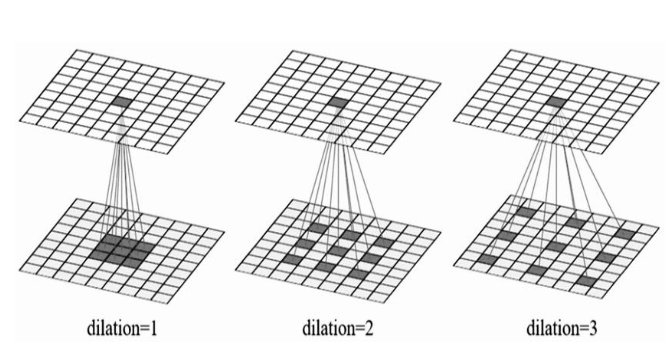
\includegraphics[width=\linewidth]{tikz/dilation.png}
    \caption{{\color{red}\colorbox{pink}{Tikz TO-DO}} The image shows three convolutional filters using three different dilation rate.}
    \label{fig:dilation}
\end{figure}


In Section 5, we introduced CNN architecture, focusing on the traditional convolutions, which have a dilation rate of 1, meaning that the kernel considers adjacent pixels. 

Unlike traditional convolutions, dilated convolutions introduce gaps between the elements of the filter. This allows the network to capture information over larger spans of the input sequence. For instance, with a dilation rate of 2 (skipping 1 pixel) or 3 (skipping 2 pixels), as shown in Figure \ref{fig:dilation}, we achieve the same number of features in the next layer without changing the kernel size. This approach extends the receptive field of the convolutional filter, enabling it to incorporate more context from the input data while maintaining the computational efficiency of the original kernel size.


\section{Convolutional Sequence Model}

Convolutional Sequence Model, also called \textbf{Temporal Convolutional Network} (TCN), was the first architecture to apply the CNN to sequence processing. It marked the shift from RNN to CNN for sequence input problems.



\begin{figure}[!htbp]
    \centering
    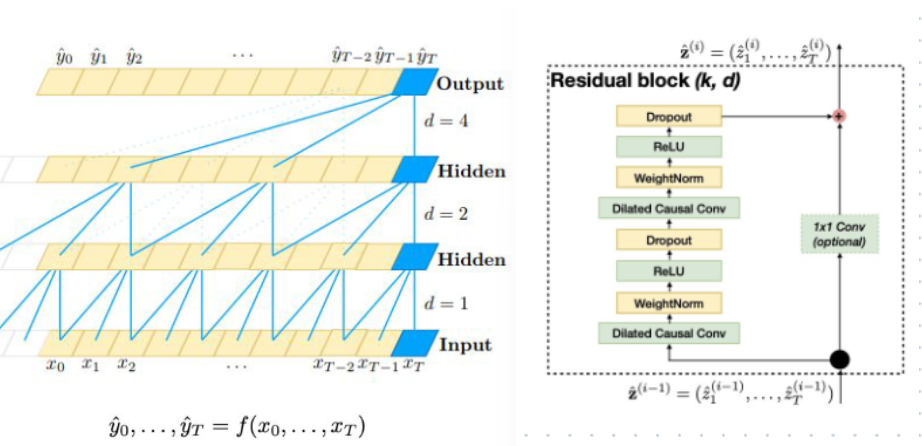
\includegraphics[width=\linewidth]{tikz/TCN.png}
    \caption{{\color{red}\colorbox{pink}{Tikz TO-DO}} \textbf{Left}: A global overview of Dilated Causal Convolution. The architecture differs a lot from the standard CNN as the output of each hidden layer is obtained by using dilation (1,2,4) and a kernels of size 3. The most relevant change is the causal effect: the CNN has been adapted to predict the tokens sequentially. For example, the output $y_t$ is predicted after $y_{t-1}$ only by using a \underline{shifted} number of features from the previous layer, namely $x_t, x_{t-4}, x_{t_8}$; \textbf{Right}: a global look to Temporal Convolutional Layer, where also residual blocks, ReLu, Dropout and Weight Normalization layers are employed.}
    \label{fig:TCN}
\end{figure}



The distinguishing characteristics of TCNs are:
\begin{enumerate}
    \item \textbf{Sequence Length Preservation}: The architecture can take a sequence of any length and map it to an output sequence of the same length.
    
    \vspace{1 pt}
    \item \textbf{Causality in Convolutions}: The convolutions in the architecture are \textbf{causal}, ensuring that there is no information "leakage" from the future to the past.
\end{enumerate}

To achieve sequence length preservation, TCNs use a 1D fully-convolutional network (FCN) architecture, where each hidden layer is the same length as the input layer. Zero padding of length (kernel size − 1) is added to maintain the length of subsequent layers, ensuring they match the length of previous ones.

For maintaining causality, TCNs employ \textbf{dilated causal convolutions}. Additionally, \textbf{residual connections} are used to enhance the learning process.

\textbf{Dilated Causal Convolution}: is a 1-dimensional convolution operation where the output at time t is computed using elements from specific input locations of the previous layer, determined by the dilation rate. This method ensures that each output only depends on specific past inputs, respecting the causality constraint.

This convolution operation is crucial for capturing temporal dependencies in sequential data, as it ensures that predictions are based solely on past information, preventing any "leakage" of future information to past data (see Figure \ref{fig:TCN}).


To put it simply, a $TCN= \text{1D FCN} + \text{ Dilated Causal Convolution layers} $.

Furthermore, the model uses relu as activation function and dropout as regularization. Additional tricked was used, which is weight normalization block.

\textbf{Weight normalization}: The layer normalizes the wieght vector, accelerating convergence without introducing dependencies between examples in a minibatch (that is the reason why it was used).


Their findings demonstrated that leveraging these elements enhances the effectiveness of the CNN across various sequence modeling tasks compared to traditional RNNs like LSTMs.



\section{Convolutional Seq2Seq learning}
This paper adopts Google's Seq2Seq learning model and introduces a CNN-based approach. Let's consider the task of translating a sentence from German to English.

In the original Google architecture, the encoder consists of a Bidirectional LSTM. Its output is concatenated to form the input for subsequent layers. This concatenated output is then used to construct a self-attention mechanism, which captures important relationships within the input sequence. Subsequently, the decoder predicts the English translation using the latent representations associated with the concatenated output and attention mechanism.

However, in this paper, researchers replaced the Bidirectional LSTM in the encoder with a Temporal Convolutional Network (TCN), which produces latent representations used for attention computation. Additionally, the decoder is transformed into a CNN-based architecture too. Gated Linear Units and residual connections are employed in both the encoder and decoder.

The CNN-based decoder enhances training efficiency by leveraging parallel computing capabilities.

\begin{figure}[!htbp]
    \centering
    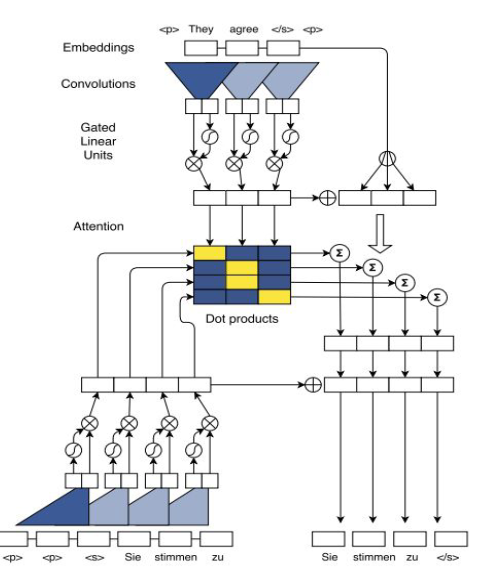
\includegraphics[width=\linewidth]{tikz/Convolutional Seq2Seq.png}
    \caption{{\color{red}\colorbox{pink}{Tikz TO-DO}} A global view of Convolutional Seq2Seq architecture}
    \label{fig:C-Seq2Seq}
\end{figure}


\section{Attention is all you need}

The paper "Attention is All You Need" revolutionized NLP research by introducing the Transformer model, which uses only fully connected layers and attention blocks for Neural Machine Translation (see Figure \ref{fig}).

\textbf{Transformer}: A Transformer model transforms one sequence of input into another based on a specific task. For example, it can translate text from English to Italian or generate an answer to a question. It uses an Encoder and Decoder stacked together. Unlike CNNs and RNNs, the Transformer doesn't rely on a recurrent structure for encoding and decoding. Instead, it uses attention mechanisms to focus on all parts of the input sequence simultaneously at each decoding step. This parallel processing speeds up both training and inference, making it great for handling long sequences and complex dependencies.


At its core, A Transformer model predicts new words by combining the source sentence and the already predicted target words. The source sentence is fed into the encoder's \textbf{input embedding}, while the target sentence is fed into the decoder's \textbf{output embedding}. Both are then combined to determine the probability of the next word. For example, when translating the third word, the model considers the entire source sentence ("the cat eats the mouse") and the target sentence produced so far ("il gatto" in Italian). 

Now, let look closer to each component of the transformer (see figure \ref{fig:transformer}).


\begin{figure}[!htbp]
    \centering
    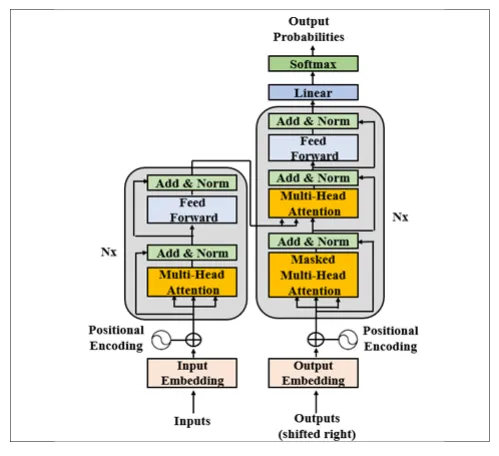
\includegraphics[width=\linewidth]{tikz/transformer.jpg}
    \caption{{\color{red}\colorbox{pink}{Tikz TO-DO}} A gloabl view of transformer architecture. \textbf{Left-hand side}: encoder}
    \label{fig:transformer}
\end{figure}

\subsection{Encoder}


\textbf{goal}: The Encoder's goal is to view the entire input sequence at once and determine which tokens are important in relation to others using the Attention Layer. This layer creates modified input embeddings that reflect this 'attention'.



After having explained the purpose and function of the encoder, we will break down each step to understand how the encoder produces its output. We KINDLY suggest to see figure references while reading. Hold on tight and lets go!

\begin{figure}[!htbp]
    \centering
    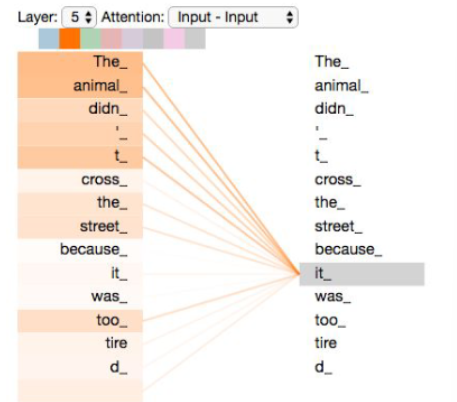
\includegraphics[width=\linewidth]{tikz/Encoder Goal.png}
    \caption{{\color{red}\colorbox{pink}{Tikz TO-DO}} The image visually illustrates the encoder's output. For a word in the input sequence, such as "it", the encoder captures the context of other relevant words in the sequence (attention).}
    \label{fig:encoder-goal}
\end{figure}

\subsubsection{Step 1: Setting up the Input Sequence}

(Step 1.1): Starting from the bottom of the structure (left-hand side of figure \ref{fig:transformer}), we first encounter the \textbf{input sequence} (source sequence). As seen in appendix \ref{sec: word-emb}, we generally feed the encoder with a \textbf{numeric representation} (not embedding) of the sequence. Say, we aim to convert ‘I am a boy’ to German. We can't use text directly but instead a numeric representation  for each token (I, am, a, boy) is generated using a \textbf{tokenizer}.

(Step 1.2): The tokenized sequence undergoes an \textbf{Input Embedding} layer, producing \textit{meaningful embeddings}\footnote{similarity between words. for example, "children" and "child" would have similar embeddings, while "children" and "cat" would no} of dimension 512 for each token. For instance, the phrase "I am a boy" may be represented numerically as [1, 2, 3, 4], with each token mapped to a 512-dimensional vector. 

(Step 1.3): \textbf{Positional Encoding}: Since the meaning of a word depends not only on its semantic content but also on its position within the sequence,\footnote{For example, consider the sentences: "He has a black Ferrari" and "He also has a white cat". If we only use the Input Embedding Layer, both ‘black’ and ‘white’ will have similar embeddings (as they are adjectives). However, in the first sentence, these words are far apart and relate to different entities.} we need to \textbf{add} relative position information of each token to the embedded input sequence. With positional encoding, the model learns that words are similar based on their meaning (e.g., child and children) and their relative position in the sentence (e.g., an adjective usually comes before a noun).

This layer has the following characteristics:
\begin{itemize}
    \item It is added at the bottoms of both the encoder and decoder stacks (we will see later). 
    \item It has the same dimension as the embeddings ($nx512$), so that the two matrixs can be summed.
    \item  each dimension of the positional encoding corresponds to a Sinusoidal embedding. 
\end{itemize}

Although not necessary, let's look at the equation used to compute the positional information to better understand how it works:

\begin{equation}
        & PE _{(\text{pos} 2i )} = \sin{(\frac{pos}{1000^{\frac{2i}{d_{model}}}})} \\
        & PE _{(\text{pos} 2i+1 )} = \cos{(\frac{pos}{1000^{\frac{2i}{d_{model}}}})}   
\end{equation}

This formula means that for every token at index ‘pos’ in the ‘input embedding’ layer (pink box in Figure \ref{fig
}), we generate a positional vector of dimension 512. For every even embedding index (0, 2, 4, 6, ..., 510), we use the first formula; for odd indexes (1, 3, 5, 7, ..., 511), we use the second formula.

For example, to generate the positional encoding for ‘boy’ in the sentence "I am a boy" (where pos = 4), if the corresponding original embedding is [1.2,3.2,...,1.1][1.2,3.2,...,1.1] of size 1×512, the positional vector will be of size 1×512:

$$\left[
[\sin(\frac{4}{1000^0}), \cos(\frac{4}{1000^0}), \sin(\frac{4}{1000^4}), \cos(\frac{4}{1000^4}), \ldots, \cos(\frac{4}{1000^{1022}})]
\right]$$

Once obtained for each token, the positional vector is added to the corresponding original token embedding (see Figure \ref{fig:transformer})


\subsubsection{Step 2: Inside the Encoder}

Once the input sequence has been properly embeeded, it goes through the core of the encoder. The encoder comprises \textbf{4 segments} that are repeated for \textbf{‘Nx’ times} (Nx=6 in the paper). These components are 
\begin{itemize}\label{components}
    \item Multi-Head Attention
    \item Add And Norm
    \item Feed Forward Neural Netwrok
    \item Add and Norm
\end{itemize}

Let us dive into each of the 4 components one by one.

\paragraph{Multi-Head Attention Layer} 

Remember that attention layer makes our model focus on important words of a sentence. For example, in ‘ I am a boy ‘, ‘am’ is of not the same importance as of ‘boy’ when it comes to understanding the meaning of the sentence. 


A Multi-Head Attention Layer can be considered a \textbf{stack} of parallel Self-Attention Layers which can help us in understanding different aspects of a sentence. The keyword stack refers to the  multiple "attention heads" that are used to gather diverse perspectives on a shared question or sentence\footnote{Just as different individuals may interpret and respond to a question differently, these "attention heads" associate words or concepts differently. This enables the model to gain a more comprehensive understanding of the input text.}. 

\textbf{Each head} in the Multi-Head Attention Layer intakes the new embedding  which is $n x 512$ and produces an output of shape $n x 64$. This output from all heads is then \textbf{concatenated} to produce a single output of the dimension $n x 512$ (same as the input, but this time usefull information has been extracted). In the paper, \textbf{8 attention heads} are used.

\textbf{Key, Value and Query}

Before moving onto the attention mechanism, a few concepts need to be introduced. For each n-th embedded word, the self-attention block uses the following concepts:

\textbf{Query}, \textbf{Key} and \textbf{Value}, which are 3 vectors for each input embedding computed by multiplying the input embedding with 3 weight matrices, learned during training.  \textbf{Query}, \textbf{Key} and \textbf{Value} vectors represents a specific word.

As we will see later, each \textbf{query} vector is multiplied with \textbf{all key} vectors. This operation produces a  "score" which determines how much focus the model should place on other parts of the input sentence (\textbf{keys})  we it encodes a word at a certain position (one \textbf{query}).

\begin{figure}[H]
    \centering
    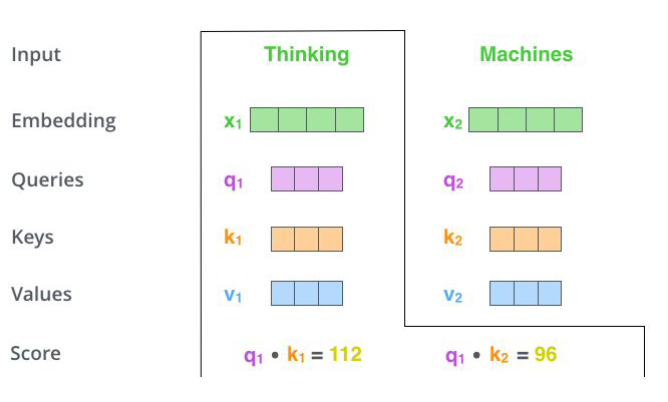
\includegraphics[width=1\linewidth]{Attention Score.png}
    \caption{Self attention for "thinking"}
    \label{fig:self attention}
\end{figure}


The idea is that when a \textbf{query} and a \textbf{key} match well, i.e, two words have similar meaning, the attention score will be high, and the corresponding \textbf{value} will be emphasized more in the output. Visually, you can think of \textbf{keys} as a bunch of vectors in space and \textbf{queries} as the best representation of a specific word the encoder is looking for. If the two vectors are close, their dot product (or the cosine similarity) will be high, indicating that the words they represent are similar (like "child" and "children").


The attention layer uses these vectors for each embedded word in the input sequence, thus we have 3 matrices pair, \textbf{Query}, \textbf{Key} and \textbf{Value}, each of dimension $n \text{ x } d_k$, where $d_k = 64$.

As stated at the begging, this matrices are obtained by multiplying the input embedding with 3 weight matrices, namely \textbf{Query weights}, \textbf{Key weights}, \textbf{Value weights}, each of dimension $d_{model} \text{ x } d_v = 512x64$.
    


\paragraph{Self-Attention}
We have all the ingredients for understanding self attention.

\textbf{Self-Attention is a mechanism for creating arbitrarily long-range weighted dependencies between word tokens in language models}.

The selfe-attention is computed for \textbf{each token} in the sequence with the formula below:

\begin{equation}\label{eq: attention}
    \text{Attention}(Q,K,V) = \text{softmax}(\frac{QK^T}{\sqrt{d_k}})V
\end{equation}

To explain the formula, let's use just one embedded word and compute its self-attention.

The first term computes the dot products between $ q_1 \cdot K^T$. As we are only considering the first token (first row $q_1$ of Query matrix ), we obtain a vector of $1xn$ where each element represents the score that determines \textbf{how much focus to place on other parts of the input sentence as we encode this word}. Repeating this process for all remaining rows of the Query matrix, we obtain an output of $nxn$.

The formula then uses a normalization factor, $\sqrt{d_k}$, to maintain stable the computations and thus the gradient. It then applies the softmax along rows. Words will have an high score if they are someone related to the word at this position. 

Finally, we multiply \textbf{ the softmax score vector} (still for the first word) by \textbf{each Value vectors}, obtaining an output of $nxd_k$. This is done to keep intact the values of the words we want to focus on and drown-out irrelevant words. After summing up the weighted
value vectors, we obtain \textbf{the output of the self-attention layer at this position} ($1xd_k$). We repeat this process for all softmax score vectors and the final output will be $nx d_k$.

\begin{figure}[H]
    \centering
    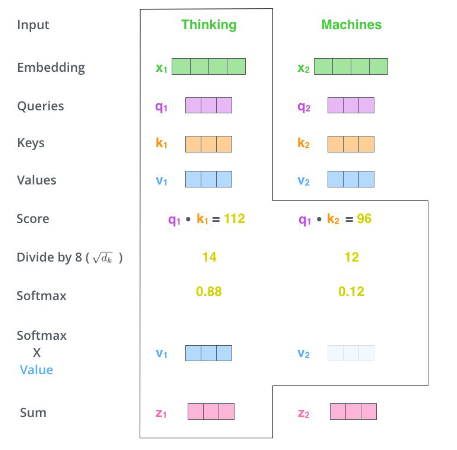
\includegraphics[width=0.75\linewidth]{tikz/Self Attention.png}
    \caption{An example of self attention}
    \label{fig:self-attention}
\end{figure}

Applying the produces for every word, the output of the layer will be an  Attention matrix  of  shape $n x d_k$. It is a differentiable output that can be learnt during backpropagation.
As we have 8  attention heads, once we compute the attention matrix for each,  we then concatenate them together, $n \text{ x } d_{model}$. The very last step is to  multiply the concatenated matrix with a weights matrix. \textbf{The output of the Multi-Head Attention is obtained}.

\begin{figure}[H]
    \centering
    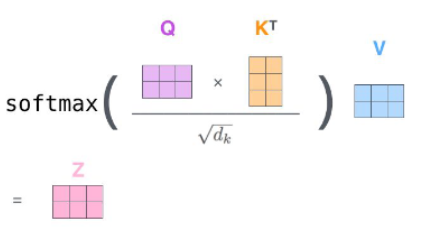
\includegraphics[width=0.5\linewidth]{tikz/Attention formula.png}
    \caption{{\color{red}\colorbox{pink}{Tikz TO-DO}} A visual representation of equation \ref{eq: attention}}
    \label{fig:attention-formula}
\end{figure}

\begin{figure}[H]
    \centering
    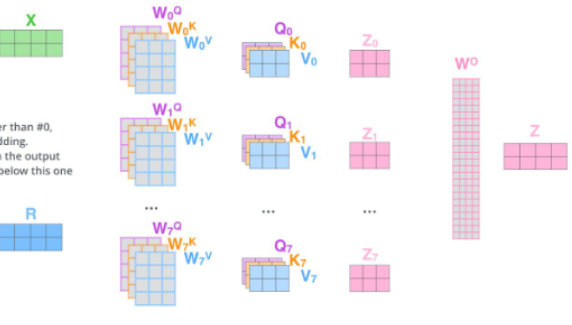
\includegraphics[width=\linewidth]{tikz/Attention block breakdown.png}
    \caption{{\color{red}\colorbox{pink}{Tikz TO-DO}} A visual representation of attention block, broken down into each pices of equation \ref{eq: attention}.}
    \label{fig:attention-block-breakdown}
\end{figure}


\paragraph{Example}

Let's see a shallow example to better understanding what goes on inside the attention mechanism.

Let's assume we have an input sequence like ‘Black and Brown’.

Step 1: We pass the input phrase into the tokenizer, which produces an output of $3x4$, where the number of tokens is $n=3$ and each has dimension $d_{model} = 4$. In the image below we can see how the Positional Encoding is generated for words ‘Black’ and ‘Brown’ (\textbf{A}:). Each row of the matrix represents the Positional Encoding of each token of the input sequence (\textbf{B}). We then initialize the  Query, Key and Value weight matrices, which have same dimension $4x3x3$ ($d_{model} x d_{w}x 3$)(\textbf{C}). Thus, $d_k,d_v, d_q = 3$.

\begin{figure}[H]
    \centering
    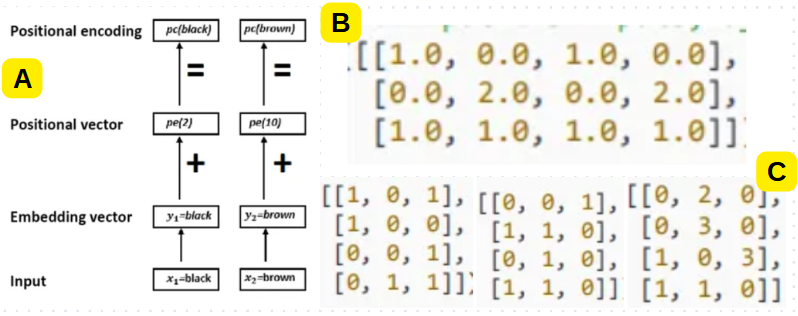
\includegraphics[width=\linewidth]{tikz/Attention Example 1.png}
    \caption{{\color{red}\colorbox{pink}{Tikz TO-DO}} }
    \label{fig:transformer-input-embedding}
\end{figure}


Step 2: as can be seen in the figure belowm we pass the positional embedding matrix in as Input to the Multi Head Attention layer, using the initialized weight matrices. The \textbf{left} figure represents of attention block operations, lets break them down. 

Each row of Input Embedding represents a token of the input sequence. Row 1 represent Black, Row 2: and, Row 3:Brown. Next step we multiply the input with $Q_w, K_w,  V_w$ respectively. We get the output Query, Key and Value matrix  of dimension 3X3x3 ($n x d_{model}$x3) showed in the \textbf{right}  figure. The order is Q, K, V and each row corresponds to Query, Key and Value for each one of the input sequence tokens.

\begin{figure}[H]
    \centering
    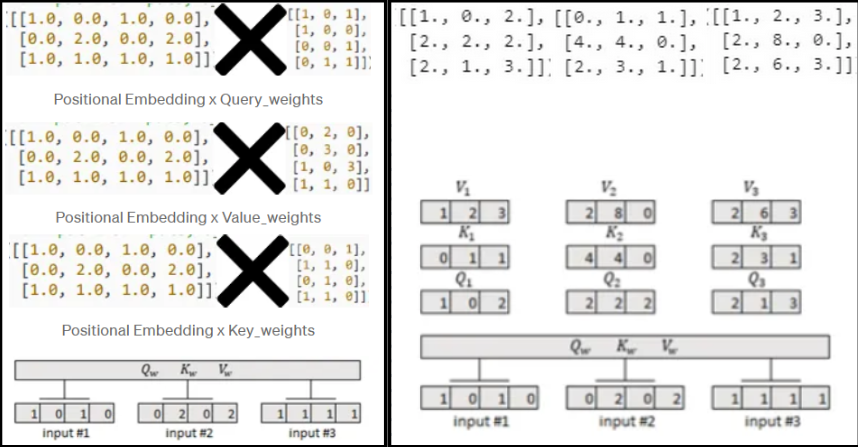
\includegraphics[width=\linewidth]{tikz/Attention Example 2.png}
    \caption{{\color{red}\colorbox{pink}{Tikz TO-DO}} }
    \label{fig: transformer-attention-block}
\end{figure}



Then, we compute attention with equation \ref{eq: attention}. We have shown in the example the computation for the 1st token(\ref{}). 

First, we have to multiply the values of the first row (first token) of the Query matrix with all the rows of the Key matrix, obtaining a vector of $1x3$. Figure \textbf{C} shows the computation for all the tokens, where each row represents one token ($nxd_k$).

Second, we normalize (skipped in this case to make an easier example) and the compute the softmax by row. Figure \textbf{B} show the softmaxed values for all the tokens, where each row represents one token. \textbf{The softmaxed scores for a token represent the importance of tokens corresponding to other tokens}. For example, Softmaxed score for 1st token ‘Black’ =[0.06,0.46,0.46] implies the Importance of ‘Black’ for Black=0.06, and=0.46, Brown=0.46.

Third, we multiply each softmaxed value with Value matrix, obtaining for each row (token) an output of $n x d_{k}$, thus the final output will be $n x d_{k}x3$. This is showed in figure \textbf{A} for the first token in the "Attention (Q,W,V) values for input #1" block.

The last step is to compute the attention values for each token. This is made by summing up along rows of each token's matrices, obtaining for each token a vector of $1x d_k$, thus the final output will be a matrix of $nxd_k$. Figure \textbf{A} shows the attention values for 1st token, which are retrieved by summing along row of matrix contained in "Attention (Q,W,V) values for input #1" block.

Similarly, we can calculate attention for the remaining 2 tokens (considering 2nd and 3rd row of softmaxed matrix respectively) and hence, our Attention matrix will be of the shape, $n x d_k$ i.e. 3 x 3 in our case.





\begin{figure}[H]
    \centering
    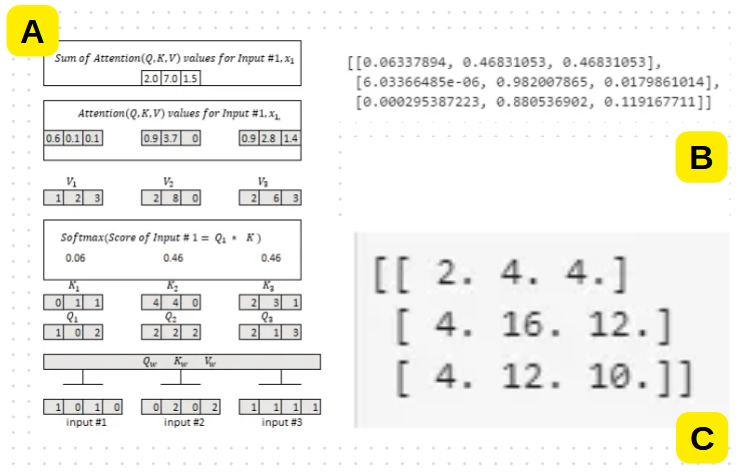
\includegraphics[width=\linewidth]{tikz/Transformers Example 3.png}
    \caption{{\color{red}\colorbox{pink}{Tikz TO-DO}}}
    \label{fig:transformer-attention-softmax}
\end{figure}

\paragraph{Post Layer Normalization and FF layer}

To ensure no essential information is lost, \textbf{normalization layer} and \textbf{residual connections} are used to simultaneously in each sub-layer of the encoder, namely the Self attention and the Fully connected layer. The normalized Multi-head's output is fed into a Feed-Forward Network comprising of 2 layered neural networks applying ReLU. 
 
For example, in the Multi-Head attention, this is achieved through the following steps:

\begin{enumerate}
\item Add the input and output of the Multi-Head Attention Layer.
\vspace{0.5 pt}
\item Apply \textbf{Layer Normalization}.
\end{enumerate}


\begin{figure}[H]
    \centering
    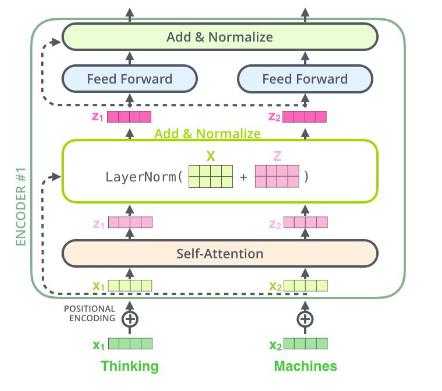
\includegraphics[width=0.75\linewidth]{tikz/Residula in Transformers.png}
    \caption{An example of residual blocks and normalization layer in Transformers}
    \label{fig:Residual-NormLayer}
\end{figure}



\subsubsection{Step 3: Final}

Now, the 4 encoder segments (section \ref{components}) are repeated for 6 iterations ($Nx$).

The final output from the second Normalization Layer in the 6th iteration has dimensions $n×d_{model}$ and is passed to the \textbf{Decoder} as the \textbf{attention matrix} for the input sequence. We will discuss how this is integrated into the decoder in the following explanation.

\subsection{Decoder}
    

The primary aim of using a Decoder is to determine the tokens of the output sequence one at a time by leveraging:

\begin{itemize}
\item Attention scores for all tokens in the input sequence retrieved from the Encoder (last iteration).
\item All predicted tokens of the output sequence up to the current point.
\item Once a new token is predicted, it is used to determine the next token. This process continues until the 'End Of Sentence' token is predicted.
\end{itemize}

As with the Encoder, we will explore this network using a bottom-up approach (see figure \ref{fig:transformer}).

\subsubsection{Step 1: Outputs}

Outputs represents the numeric representation of the Output Sequence generated so far. As done with the Encoder, we employ a tokenizer but with a difference. This numeric representation is \textbf{right-shifted}.

The reasons behind this choice is due to the fact that the decoder predicts the next word of the sequence given the previous predicted tokens and attention from Encoder. Now, for the 1st token, this looks troublesome as there exist no previous tokens. Hence, the output sequence is shifted and a ‘BOS’ (Beginning of Sentence) is inserted at the beginning.


(step 1.1 and 1.2): The Output Embedding and Positional Embedding layers have the same role and structure as in Encoder.

\subsubsection{Step 2: Masker Multi-Head}

In Masked Multi-Head Attention Layer, attention is applied on tokens \textbf{up to current position} (index till which prediction is done by transformer) and not future tokens (as aren’t predicted till now). This is in stark difference from Encoder where attention is calculated for the entire sequence at once.

For example: If we wish to translate ‘Drug is good’ (input for the encoder, attention will be calculated for all tokens all at once) into French i.e ‘drogue est bonne’ (input for decoder) and the translation has reached till ‘est’(2nd token), hence, ‘bonne’ would be masked & attention will be applied for the 1st 2 tokens. This is done by setting future tokens (embedding for ‘bein’) as infinite values


After this, Residual conntection and Normalization Layer same as in Encoder is followed.

\subsubsection{Step 3: use the Encoder Output}

After the Normalization layer, a \textbf{Multi-Head Attention} layer follows which:

\begin{itemize}
    \item Intakes the output from Encoder ($n x d_{model}$), calls this output K and V, which are used as Key and Value by \textbf{Decoder’s Multi-Head Attention}.
    \item Uses the \textbf{Query matrix} from the previous Masked Multi-Head Attention layer is taken. Hence, this attention layer doesn’t require \textbf{any training} as takes pre-trained values for Query, Key and Value matrices.
\end{itemize}

After this layer, Redisual connection, Normalization, FFNN and Normalization layers come and the whole procedure is repeated 6 times ($Nx$). \textbf{The last iteration computes the final output of the decoder}.

\subsubsection{Step 4: Prediction}

After these repeated code blocks, we have a linear layer followed by a \textbf{softmax function} giving us the probability for the aptest token in the predicted sequence.

Once the most probable token is predicted, it goes back in the tail of the output sequence.

\subsection{Conclusions}

The Transformer architecture has demonstrated competitive against established RNN and CNN structures. Nonetheless, its training costs are notably reduced owing to the Self-Attention Layer's ability to compute attention with \textbf{all the words in same sentence at once}. Consequently, computations primarily entail matrix multiplications, a computationally less demanding task that lends itself well to parallelization. Despite its superior performance in handling long sequences, in order to  extract diverse meaningful representations multiple attention heads are needed, which leads to parameter explosion, thereby posing a significant challenge.

Also, after transformers took place and became the SOA, the community started to develop models employing just the encoder or decoder model alone. The first category  uses only the output hidden states, which can be incorporated as features in other model for performing different tasks (BERT). The second are created for text generation, which make them suitable for tasks like machine translation or summarisation (Transformer XL or GPT series).

\section{Vision Transformer (ViT)}

The previous CNN were limited by the notion of the \textbf{receptive field}. The Receptive field of neuron  of layer $j$ w.r.t layer $j−1$ is the
region of layer $j−1$ that neuron $j$ has access to in order to produce its activation. Thus, the receptive field of a CNN is strictly dependent on the kernel size of the given convolutional layer, hence it limits its power.

Vit expanded convolution capacity by applying the self-attention concept to images, thus shifting the Transformer models from NPL to Computer vision. It is basically the attention is all you need applied to images, i.e. 3-dimensional data instead of 2.

\begin{figure}[H]
    \centering
    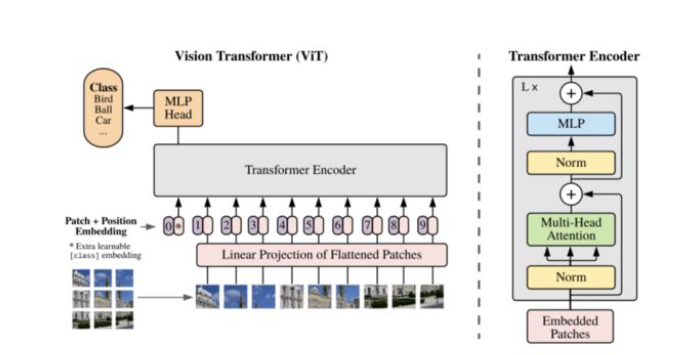
\includegraphics[width=\linewidth]{tikz/ViT.png}
    \caption{{\color{red}\colorbox{pink}{Tikz TO-DO}} The image shows an overview of the ViT architecture. The cells in grey are the positional embeddings, whereas those in pink are the \textbf{class tokens}.}
    \label{fig:ViT}
\end{figure}

Recall that self-attention is a mechanism for building \textbf{semantic
long-range learnable relationships}. In this case, the phrase can be transformed into \textbf{learning the relationships between pixels of a fixed size areas of the image}.
The main difference of self attention in respect of NPL is that, in computer vision, \textbf{self-attention} is used to model the
self-similarity within images\footnote{For example, if the background of an input image there are two cars, the areas encompassing these object will be detected as similar.}.

Thus, in order to pass an image input into the encoder, it is splitted into patches premilinary deciding the number of division.

The input (as patches) is embedded in a lower dimension to reduce
complexity (through special algorithm). Furthermore, ViT attaches an additional learnable embedding called \textbf{class token}.

\textbf{Class Token}: The Class token is an embedding vector that is randomly initialized and learned during the training process. It is added at the beginning of the sequence of embedded patches. It serves to gather global information from the image through the transformer's self-attention mechanism. At the end of the process, the class token is used to perform the final classification of the image.



The MLP head only looks at data from the last layer’s Class Token and no other information.




\subsection{Results}
When trained on mid-sized datasets such as ImageNet, such models yield modest accuracies (few points below ResNets of comparable size).

Transformers lack some of the inductive biases inherent to CNNs,
such as translation equivariance and locality, and therefore do not generalize well when trained on insufficient amounts of data.

However, the picture changes if the models are trained on larger
datasets (14M-300M images).

\section{Swiss Transformer}

Swiss transformer builds hierarchical feature maps by merging image
patches in deeper layers. It has dynamic partitioning that allows to retrieve better localized representations. Furthermore, it has a linear computation complexity to input image size due to computation of self-attention only within each local window.

It can serve as a general-purpose backbone for both image classification and dense recognition tasks.

\begin{figure}[!htbp]
    \centering
    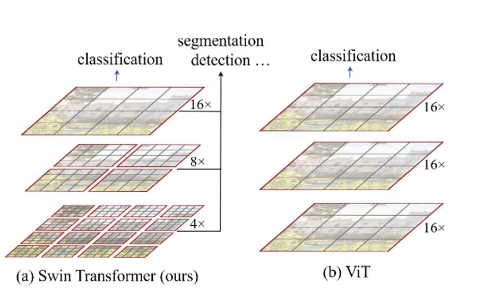
\includegraphics[width=\linewidth]{tikz/Swin Transformer.png}
    \caption{{\color{red}\colorbox{pink}{Tikz TO-DO}} The image shows the comparison between Swin transformer and Vit when computing the self-attention. Swin computes self-attention in sub areas. In layer $l$, a regular window partitioning scheme is adopted, and self-attention is computed within each window. In the next layer the window partitioning is shifted, resulting in new windows. The self-attention computation in the new windows crosses the boundaries of the previous windows in layer $l$, providing connections among them.}
    \label{fig:Swin-transformer}
\end{figure}